\chapter{Magma Dynamics: porosity waves}
\label{cha:porosity-waves}

\section{Problem Overview}
\label{sec:porosity_waves-formulation}


While many modeling packages in Earth science solve for thermal or
thermo-chemical convection,  one of the strengths of \TF{} is that it
is not a ``convection code'' or a ``magma code'', but rather a general finite element PDE
solver and can be used to model arbitrary problems as long as the weak
forms are well posed.  In particular,  \TF{} was primarily designed to
explore coupled fluid/solid mechanics with a primary application area
being the flow of magma and fluids in the deep earth.  A more general
theory of magma dynamics has been derived by multiple authors
\cite{mckenzie_generation_1984,scott_magma_1984,scott_magma_1986,spiegelman_flow_1993,spiegelman_flow_1993-1,bercovici_two-phase_2001-1,bercovici_energetics_2003,simpson_multiscale_2010,simpson_multiscale_2010-1}
that considers the flow of a low viscosity fluid in a viscously
deformable solid matrix.  From the beginning of magma dynamics,  one
of the intriguing features of these models is that they admit
dispersive non-linear magmatic
solitary  waves that propagate through the solid as ``hump
shaped'' blobs with radial symmetry that propagate at a characteristic
speed $c$ that depends on amplitude, dimension and material
parameters.  Figure \ref{fig:SolitaryWavesAllD} shows some example
solitary wave profiles for 1,2 and 3-D solitary waves that all
propagate at the same speed $c=5$ times the melt velocity in the
background constant porosity region.  

\begin{figure}[htb!]
  \centering
  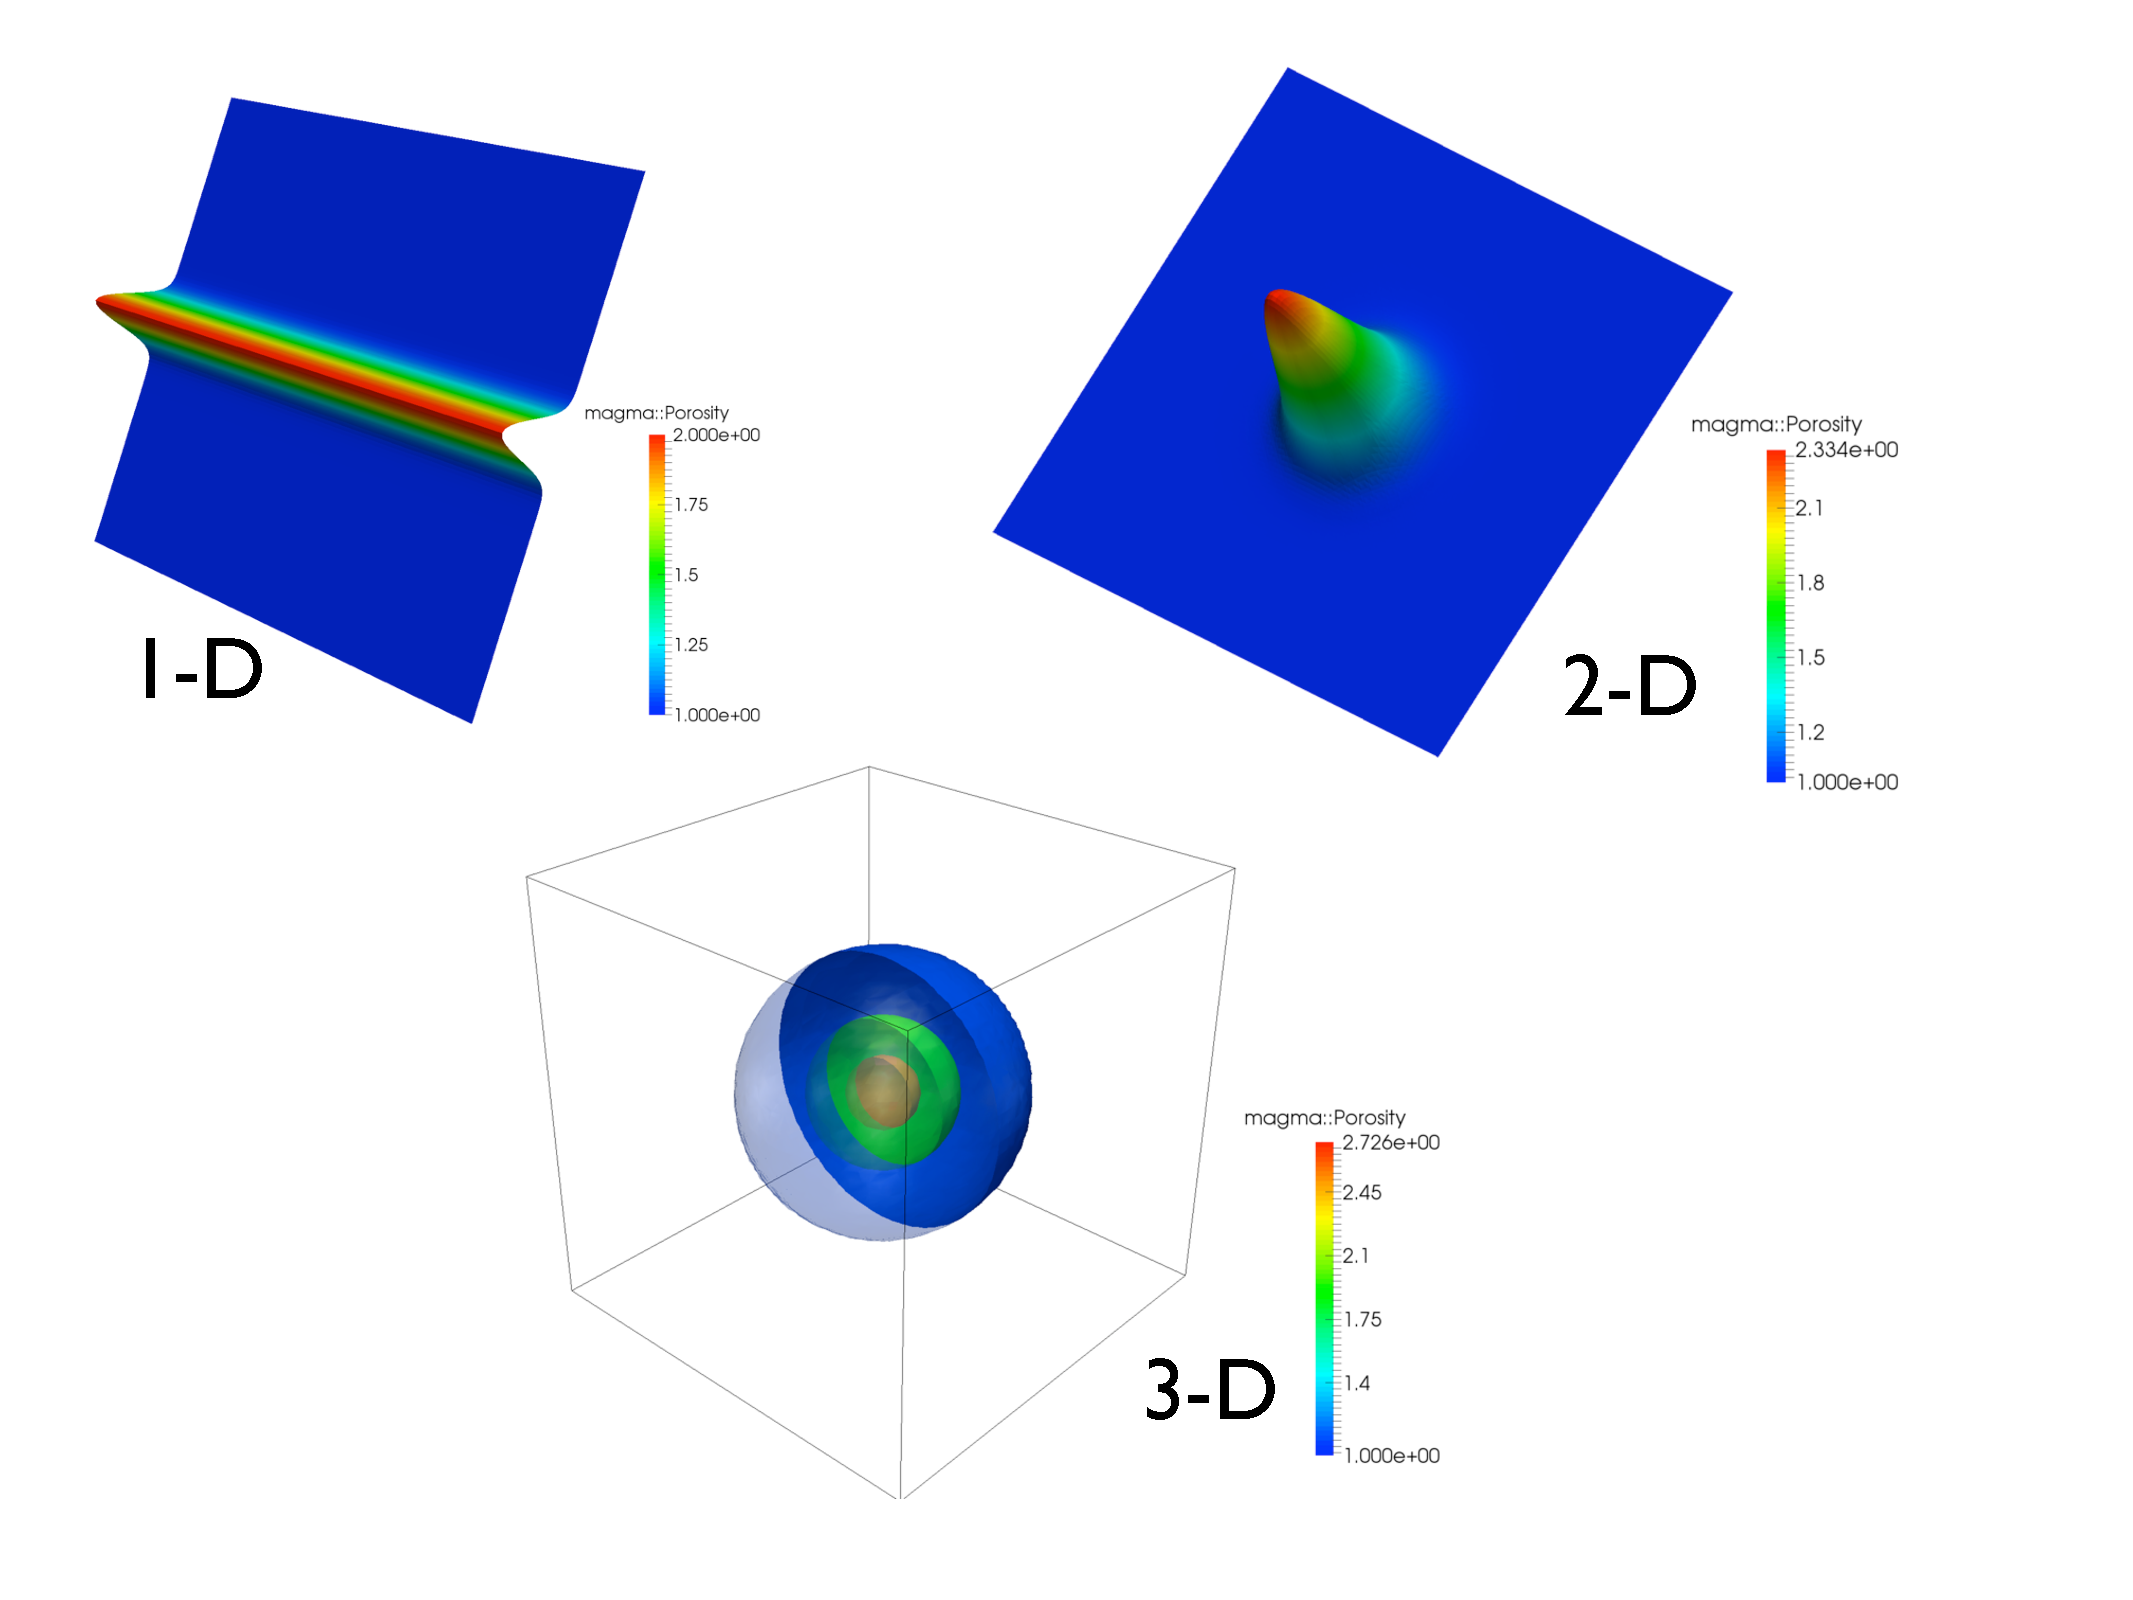
\includegraphics[width=.8\textwidth]{figures/CompositeSolitaryWaves.pdf} 
  \caption{example 1,2 and 3-D magmatic solitary waves that all move
    at speed $c=5$ times the background porosity.}
  \label{fig:SolitaryWavesAllD}
\end{figure}

In the limit of small porosity, the dimensionless governing equations for evolution
of porosity $\phi$ and ``compaction pressure'' $\pcmp$ in a frame
moving at a constant velocity $\Vs$ can be written
\begin{gather}
  \ppt{\phi} + \Vs\cdot\grad\phi = 
  \left(
    \frac{h}{\delta}
  \right)^{2}\frac{\pcmp}{\zeta}  \label{eq:5.1}\\
-\div K \grad\pcmp + \left(
    \frac{h}{\delta}
  \right)^{2}\frac{\pcmp}{\zeta} = \div K \ghat    \label{eq:5.2}
\end{gather}
where $K=\phi^{n}$ is the permeability, $\zeta = 1/\phi^{m}$ is the
bulk viscosity, $\ghat$ is the unit vector in the direction of
gravity.  These equations are scaled by an arbitrary lengthscale $h$
(usually the system height), in which case  $(h/\delta)$ is  the
system height  in compaction lengths
\begin{gather}
  \delta = \sqrt{\frac{K_{0}\zeta_0}{\mu}}
\end{gather}
The compaction length is the intrinsic length scale over which
pressure variations due to obstructions in melt flux propagate as
viscous stresses in the matrix. (See
\cite{spiegelman_flow_1993,spiegelman_flow_1993-1} for more
details). In the limit the compaction length is much bigger than $h$,
these equations reduce to Darcy flow in a rigid, but translating medium.

Equations (\ref{eq:5.1})--(\ref{eq:5.2}) form a coupled
hyperbolic/elliptic set of equations for the evolution of porosity and
pressure.  For an arbitrary initial condition, these equations will
break up into a series of localized solitary waves that propagate at a
constant speed that depends on amplitude and maintain constant shape
in the absence of collisions or mass transfer between solid and
liquid.  Remarkably, however, we can seek solitary wave solutions in
all dimensions $d$ of the form
\begin{equation}
  \label{eq:5.4}
  \phi(\vec{x},t) = f(r) = f
  \left(
    \sqrt{\sum_{j}^{d-1} x_{j}^{2} + (x_{d} -ct)^{2}}
  \right)
\end{equation}
where $r$ is the radial distance from the peak of the wave.
Substituting $f(r)$ into Equations (\ref{eq:5.1})--(\ref{eq:5.2})
transforms them into a 3rd order, non-linear ODE in $r$.  Except for
some special cases,  these ODE's do not have analytic closed form
solutions, however,  Simpson and Spiegelman
\cite{simpson_solitary_2011}, provides an elegant spectrally accurate
method for numerically calculating solitary wave profiles for all
values of $c,n,m,d$ using the ``sinc collocation method''.  Moreover,
Gideon Simpson has encoded this method in a set of python routines
\texttt{magmasinc} which have been included in this tutorial along
with a set of classes for managing and evaluating the solitary wave
profiles.  For example, the script
\texttt{\$TF\_HOME/share/terraferma/tutorials/porositywaves/python/scripts/see\_wave\_profiles.py} initializes 3 different
solitary waves for $c=5$, $n=3$, $m=1$ and $d=[1,2,3]$, using 150
collocation points.  Figure (\ref{fig:SolitaryWaveProfiles}) shows radial profiles $f(r)$ for these
3 waves.  

\begin{figure}[htbp!]
  \centering
  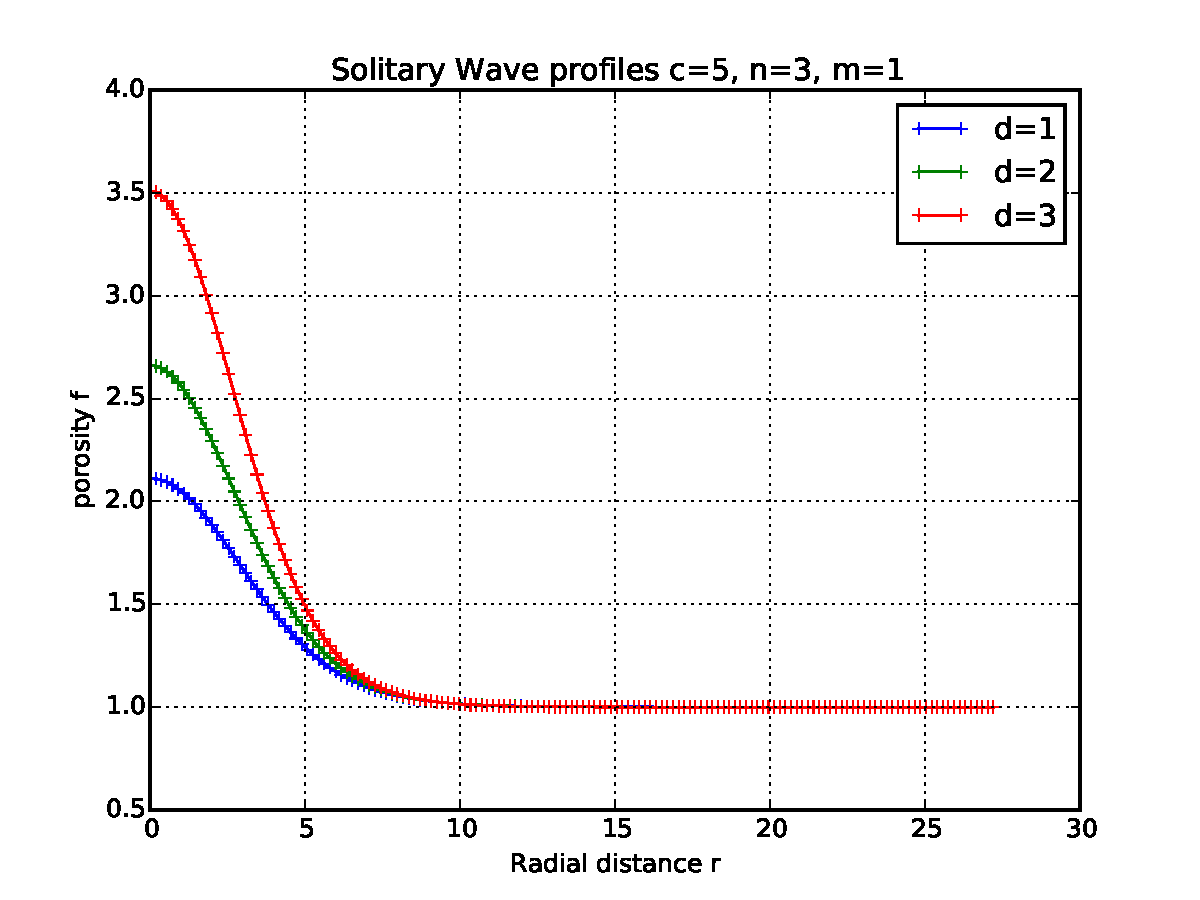
\includegraphics[width=.75\textwidth]{SolitaryWavesProfiles.pdf}
  \caption{Solitary wave profiles $f(r)$ for 1,2 and 3-D waves
    calculated using the pysolwave python package that installs with
    \TF.  All waves travel at speed $c=5$ and have permeability
    exponent $n=3$ and bulk viscosity exponent $m=1$.  Crosses on the
    profiles show the collocation points. All distances in pysolwave
    are scaled to the compaction length in the small porosity
    background ($f=1$).  I.e. these wave profiles extend about 25
    compaction lengths from the wave peak.}
\label{fig:SolitaryWaveProfiles}
 \end{figure}

\subsection{Benchmark problem}
\label{sec:benchmark-problem}

These solitary waves provide an excellent benchmark problem for
testing any model of multi-phase flow.  If chosen as an initial
condition in a frame moving at speed $\Vs = c\ghat$ they should
simply stay put and not change shape.  Any error in position or shape
is strictly due to numerical errors.  As a first problem we will
explore the solitary wave benchmarks as laid out in Simpson and
Spiegelman, 2011 \cite{simpson_solitary_2011} which have the initial
condition of  a single 2-D
or 3-D wave with its peak at the center of a unit square or cube.
$\Vs$ is set to exactly counter the wave propagation.  Boundary
conditions on porosity and pressure are shown in Figure (\ref{fig:solitarywavebcs}). 

\begin{figure}[htbp!]
  \centering
  \def\svgwidth{.8\textwidth}
  \input{solitaryWaveBCs.pdf_tex}
  \caption{Boundary and initial conditions for the solitary wave
    benchmark problem (Simpson and
    Spiegelman,\cite{simpson_solitary_2011}). Porosity and the
    separation flux normal to the top boundary are fixed at the top of
    the domain to provide  a constant input flux of 1.
  Sides are reflection and the bottom boundary condition is ``free
  flux'' which assumes that the gradient of the compaction pressure is
zero such that there is no viscous resistance to volume change on the
bottom boundary. Note, the pressure boundary conditions are all of
Neumann type,  however, unlike Poisson,  Eq.\ (\ref{eq:5.2}) is a
modified Helmholtz problem and is well-posed with all Neumann
conditions (i.e. is not singular)}
  \label{fig:solitarywavebcs}
\end{figure}


\subsection{Variational forms and Discontinuous Galerkin Porosity}
\label{sec:variational-forms}

To write out weak forms for Equations (\ref{eq:5.1}) and
(\ref{eq:5.2}) require choosing stable element pairs for porosity and
compaction pressure.  As Eq.\ (\ref{eq:5.2}) is an elliptic equation
in compaction pressure, standard continuous Galerkin elements (e.g. \Pone
or \Ptwo) have been shown to be adequate for pressure.  Moreover, In the
absence of the $\Vs\cdot\grad\phi$ term, Eq.\ (\ref{eq:5.1}) is
actually an ODE for porosity and continuous elements are also valid.
However, when the $\Vs\cdot\grad\phi$ is included, Eq.\ (\ref{eq:5.1})
becomes a hyperbolic equation for the evolution of porosity in a frame
moving with the solid which can present significant challenges for
accurate solution using continuous Galerkin finite elements.  This term, which
represents advection of porosity by the solid phase is actually
expected for most magma dynamics problems where there is a non-trivial
background flow of solid, such as at a mid-ocean ridge or subduction
zones, and we use it here in the benchmark problem to ``freeze'' the
solitary wave in the box by having the background flow exactly balance
the wave speed $c$.  After some trial and error, we found that using
discontinuous Galerkin elements for porosity works well\footnote{An
  alternative approach is to use Semi-Lagrangian methods which do not
  expressly include the $\Vs\cdot\grad\phi$ term and can be
  implemented in \TF{}.  However, the semi-Lagrangian capability is
  not parallel and we have found, in the end that DG is superior for
  these problems.}.  Here we
will use the mixed discrete function space $\fspace=(\Ptwo,\Ptwodg)$
where $\vec{u}\in\fspace=(p,f)$ (where $p$ will be our  \texttt{ufl}
symbol for pressure, $\pcmp$, and $f$ for porosity $\phi$).

As with the energy equation in thermal convection, we will first
discretize the time derivative in the porosity equation using finite
differences and integrate using a $\theta$ scheme (but we will simply
choose $\theta=1/2$, i.e. a second-order in time trapezoidal integration rule).  
Multiplying by appropriate test functions and integrating by parts, the
variational form of the non-linear problem can be written
\begin{quote}
  \fbox{\parbox{.9\textwidth}{Find $\vec{u}\in \fspace$ such that
      \begin{equation}
         F(\vec{u};\vec{u}_{t}) =0 
      \end{equation}
  for all test functions $\vec{u}_{t}=(p_{t},f_{t}) \in\fspace$.}}
\end{quote}
 where $F(\vec{u};\vec{u}_{t}) = F_{p} + F_{f}$ with
\begin{align}
         F_{p} =  & \int_\Omega \left(
\grad p_{t}\cdot K_{i}
                    \left[
                    \grad p_{i} + \ghat
                    \right] 
+ \chi_{i}p_{t}p_{i}
 \right])d\vec{x}  - \int_{\partial\Omega} p_{t}
                    \left[
                    K_{i}(\grad p_{i} + \ghat)\cdot\vec{n}
                    \right] ds\\
 F_{f} =& \int_\Omega f_{t}[ f_{i} -f_{n}
          -\frac{dt}{2}(\chi_{n}p_{n}+\chi_{i}p_{i})]d\vec{x}
          \nonumber\\
          & -\int_{\Omega} 
            dt\left(
            f_{1/2}\Vs\cdot\grad f_{t}
            +f_{t}f_{1/2}\div\Vs
            \right)d\vec{x}\nonumber\\
          & + \int_{\partial\Omega}dt f_{t}f_{1/2}\Vs\cdot\vec{n} ds
            \nonumber\\
          & + \int_{\mathrm{internal\,  facets}} dt [[f_{t}]]f_{1/2}^{*}\Vs\cdot\vec{n}dS\label{eq:5.5}\\
\nonumber \\
  F = & F_{p} + F_{f} \label{eq:5.systemresidual}
\end{align}
where 
\begin{align*}
  f_{1/2} = & \frac{1}{2}(f_{n} + f_{i})\\
  \chi_n = & 
             \left(
             \frac{h}{\delta}
             \right)^{2}f_{n}^{m}\\
\chi_i = & 
             \left(
             \frac{h}{\delta}
             \right)^{2}f_{i}^{m}\\
K_{i}    = & f_{i}^{n}\\
\end{align*}
are the interpolated porosity at the half-time step, bulk viscosity
terms at the old and new times and permeability at the new time. In
addition
\begin{align*}
  [[f_{t}]] = f_{t}^{+} - f_{t}^{-}
\end{align*}
is the ``jump operator'' which 
measures the difference in a function across a facet (the $^{+}$ and
$^{-}$ denote the one sided limits of the function on either side of
the facet).  For continuous elements the jump operator is zero.

These variational forms appear somewhat more complicated than those of
our previous examples for several reasons\footnote{not counting the fact, that
most people are not familiar with these equations}.  First,  the
Neumann flux boundary conditions add additional surface integrals to
the forms.  But more significantly the discontinuous Galerkin elements
for porosity add additional complexity to the variational forms for
the porosity residual.  The last three lines of Eq.\ (\ref{eq:5.5}) all arise from
integration by parts of the advective term over each element
\begin{displaymath}
  \int_{\Omega} f_{t}\Vs\cdot\grad f_{1/2} d\vec{x} = \sum_e \int_{\Omega_{e}} f_{t}\Vs\cdot\grad f_{1/2} d\vec{x}
\end{displaymath}
which generates body integrals over the domain,  surface integrals
over the external boundaries of the domain,  and because of the
discontinuous nature of the basis functions,  integrals over the
internal facets between cells.  This last term, as written, is
actually ambiguous as the porosity
$f_{1/2}$ is  multi-valued along the facets (thus the $*$ notation),
however, we still need to specify a continuous normal flux across each
facet 
\begin{equation}
  \label{eq5:flux}
    q = f_{1/2}^{*}\vec{V}\cdot\vec{n}
\end{equation}
Since, for this problem, $\vec{V}$ is already continuous, the choice
comes down to choosing an appropriate value of the porosity at the
facet. While there are many choices for this (and many are numerically
unstable), here we  will use an upwind scheme to select the
porosity from the cell that is being advected from.  Note, this is
somewhat different from a finite volume upwind scheme that uses the
cell average of the donor cell which can lead to significant numerical
diffusion.  For these problems, where the porosity is quite smooth,
this upwind scheme is quite accurate, but avoids the spurious
oscillations produced using continuous elements.

The weak form of the residual in UFL looks reasonably
similar, however, there are some additional notation required for
describing discontinuous elements.  For this problem we will actually
split the UFL into two parts.  The first is a global declaration of
some useful UFL symbols that can be used in all forms
\begin{lstlisting}[style=UFL]
# Global parameters for porosity pressure residual 
#
# permeability
K = f_i**n

#inverse bulk viscosity function
Xi_i = hsquared*f_i**m
Xi_n = hsquared*f_n**m

#porosity at a half-time step
f_half = 0.5*(f_i + f_n)

# domains for assembly of surface integrals
ds_top   = ds(4)
ds_bottom = ds(3)
ds_left  = ds(1)
ds_right = ds(2)
\end{lstlisting}
The last four lines describe some convenience symbols for the
surface integrals on the external boundaries. 

The actual UFL for the residual $F$ is then
\begin{lstlisting}[style=UFL]
#facet normal on pressure
pn = FacetNormal(p.cell())

# body integral for pressure
bp = inner(grad(p_t), K*(grad(p_i) + ghat)) + p_t*p_i*Xi_i 

# surface integral terms for fluid flux 
sptop   = -p_t*inner(ghat, pn) # force -K[grad(p) + ghat].n = 1 on top boundary
spbot   = -p_t*inner(K*ghat, pn) #"free flux BC where inner(grad(p),pn)=0

#pressure residual
Fp = bp*dx + sptop*ds_top + spbot*ds_bottom

#outward facing facet normal for porosity cell
fn = FacetNormal(f.cell())
# facet normal solid velocity
vn = dot(W, fn)
# rectified normal solid velocity ( = vn if outflow, 0 if inflow)
vnout = 0.5*(vn + abs(vn))

# body integrals for porosity
bfm = f_t*(f_i - f_n - dt*0.5*(p_i*Xi_i + p_n*Xi_n))
# body integrals for advective integrals
bfa = - dt*dot(grad(f_t), W*f_half) - dt*f_t*div(W)*f_half

# all porosity body integrals
bf = bfm + bfa

#surface integrals - external boundaries
sftop = dt*f_t*vn  # set phi=1 on the top
sfbot = dt*f_t*(vn*f_half)
sfside = dt*f_t*(vnout*f_half)  # outflows but 0 if inflow

# surface integrals over interior facets
upwindfacetflux = vnout('+')*f_half('+') - vnout('-')*f_half('-')
sffacet = dt*jump(f_t)*upwindfacetflux

# porosity residual
Ff =  bf*dx + sftop*ds_top + sfbot*ds_bottom + sfside*ds_left + sfside*ds_right + sffacet*dS

# total residual
F = Fp + Ff
\end{lstlisting}

\pagebreak{}
The key line in the above ufl are \#16--19 and  \#35
\begin{lstlisting}[style=UFL]
# facet normal solid velocity
vn = dot(W, fn)
# rectified normal solid velocity ( = vn if outflow, 0 if inflow)
vnout = 0.5*(vn + abs(vn))
...
upwindfacetflux = vnout('+')*f_half('+') - vnout('-')*f_half('-')
\end{lstlisting}
which sets the flux $q$ Eq.\ (\ref{eq5:flux}) to be the value of the
porosity from the side of the facet that is an outflow.  Note that
\texttt{vnout} evaluates to zero for an inflow facet and \texttt{vn}
the normal component of the velocity for an outgoing facet (and
\texttt{vn}$\geq 0$).

\section{Solution using \TF}
\label{sec:solution-using-tf}

While the details of the solitary wave benchmarks appear significantly
different from that of thermal convection (Chapter
\ref{cha:thermal-convection}), the structure of the problem is quite
similar and reasonably straightforward to set up in \TF{}.  We could
start with an old \texttt{.tfml} file from thermal convection but it
probably makes more sense to begin with a blank \texttt{.tfml} file
and fill it in sequentially.  Where features, such as an adaptive time
stepper, can be reused from the thermal convection problem, we will
use the (extremely useful) cut and paste functions in diamond to reuse
option blocks from other models.

A fully worked out \texttt{tfml} file for the benchmark problem 
can be found in
\texttt{\$TF\_HOME/share/terraferma/tutorials/porositywaves/benchmark/magmawaves.tfml},
along with an accompanying testharness file \texttt{magmawaves.shml}
for testing.  A typical solution is shown in Figure \ref{fig:solitarywavebcs}.

To build this model in \TF{} from scratch, do the following
\begin{steps}{Step}
  \item Make a new tfml file
  \begin{lstlisting}[style=Bash]
$ mkdir mybenchmark
$ chdir mybenchmark
$ diamond magmawaves.tfml &
  \end{lstlisting}%$
\item \textbf{Set the geometry:} Here we will use a 2-D UnitSquare mesh.
  \begin{steps}{step}
  \item Set dimension to 2 (this can only be done once)
  \item Choose \texttt{mesh (Mesh)} 
  \item Choose \texttt{source (UnitSquare)}
  \item Set \texttt{number\_cells} to $32\times32$
  \item Set \texttt{diagonal} to \texttt{right/left}
  \end{steps}
\item \textbf{Set io parameters}
  \begin{steps}{step}
  \item Set \texttt{output\_base\_name} to \texttt{magmawaves}
  \item Set \texttt{visualization->element} to (P2DG)
  \item Set dump-periods for visualization and statistics
    output.  Under \texttt{dump\_periods} 
    \begin{enumerate}
    \item Activate \texttt{visualization\_period} and set to
      0.05
    \item Activate \texttt{statistics\_period} and set to
      0.025
  \end{enumerate}
\item Activate \texttt{checkpointing} and set
  \texttt{checkpointing\_period} to 0.05.  We will need checkpoint
  files at every visualization time to be able to test the accuracy of
  the solution using an external python package.
  \end{steps}
\item \textbf{Set Time Stepping parameters}
  \begin{steps}{step}
  \item Activate \texttt{timestepping}
  \item Set \texttt{current\_time} to 0.0
  \item Set \texttt{finish\_time} to 0.5
  \item Open \texttt{timestep}
  \item Open \texttt{coefficient (Timestep)} and unfold all the way to \texttt{constant}
    \begin{enumerate}
    \item Set \texttt{ufl\_symbol (global)} to \texttt{dt}
    \item Set \texttt{value (WholeMesh)->constant } to 0.  We're
      going to use adaptive time-stepping with the initial \texttt{dt=0} trick
      that we used for thermal convection.
    \end{enumerate}
  \item Activate \texttt{adaptive} and unfold \texttt{constraint}
    \begin{enumerate}
    \item Set \texttt{constraint} name to \texttt{Courant}
      (and don't forget to hit carriage return for these name strings)
    \item Set \texttt{system} name to \texttt{CourantNumber}.  We'll
      add this system later by borrowing pieces from the thermal
      convection models.
    \item Set  \texttt{field} name to \texttt{CourantNumber}
    \item Set \texttt{requested\_maximum\_value} to 0.25 (which is
      appropriated for a $c=5$ wave and we will change this through
      the testharness as well).
    \item Activate \texttt{adapt\_period} and set to 2.0 (this won't actually try
      to re-adapt through the run giving a constant time-step)      
    \end{enumerate}
  \end{steps}
\item Unfold \texttt{global\_parameters}. Here we will set some global
  ufl symbols that can be used across all systems along with some
  dolfin specific parameters to allow parallel computation with DG elements.
  \begin{steps}{step}
  \item Activate \texttt{ufl} and in the Data box input
    \begin{lstlisting}[style=UFL]
# Global parameters for porosity pressure residual 

# permeability
K = f_i**n

#inverse bulk viscosity function
Xi_i = hsquared*f_i**m
Xi_n = hsquared*f_n**m

#porosity at a half-time step
f_half = 0.5*(f_i + f_n)

# domains for assembly
ds_top   = ds(4)
ds_bottom = ds(3)
ds_left  = ds(1)
ds_right = ds(2)
    \end{lstlisting}
(which are the same as those listed in Section
\ref{sec:variational-forms}).  Note, any changes to this global ufl
section will force a recompile of the model so use these sparingly and
with some care.  
\item Activate \texttt{dolfin} and unfold
\item Activate \texttt{ghost\_mode} and set to
  \texttt{shared\_facet}.  This will allow proper assembly of facet
  integrals in parallel (this is a dolfin parameter that we
  unfortunately need to pass through).
  \end{steps}
\item Set the \texttt{system} (and actually solve something).
  \begin{steps}{step}
  \item Set the \texttt{system} name to \texttt{magma}
  \item Choose \texttt{mesh (Mesh)} to use the defined mesh
  \item Set the \texttt{ufl\_symbol (global)} to \texttt{us}.  Again,
    this is the \texttt{ufl} symbol for the entire mixed system of
    pressure and porosity.
  \item Activate a \texttt{field}, name it \texttt{Pressure} and unfold
    \begin{enumerate}
    \item Set the \texttt{ufl\_symbol (global)} to \texttt{p}
    \item Unfold \texttt{type (Function)} and set the element to
      \texttt{(P2)} (this should automatically be \texttt{rank
        (Scalar)}
    \item Unfold \texttt{initial\_condition (WholeMesh)} and set a
      \texttt{constant} value of 0.0
    \end{enumerate}
\item Activate a second \texttt{field}, name it \texttt{Porosity} and unfold
    \begin{enumerate}
    \item Set the \texttt{ufl\_symbol (global)} to \texttt{f}
    \item Unfold \texttt{type (Function)} and set the element to
      \texttt{(P2DG)} (this should automatically be \texttt{rank
        (Scalar)}
    \item Unfold \texttt{initial\_condition (WholeMesh)} and choose
      \texttt{python}.  Now the fun begins. To use the pysolvwave
      utilities for easily generating solitary wave profiles,  we have
      written a python class \texttt{tfsolitarywave},  which reads
      parameters from a \texttt{.tfml} file (namely this one) and
      calculates solitary wave profiles.  To invoke it, add the
      following to the data window.
      \begin{lstlisting}[style=Python]
# Initialize to single solitary wave profile 
# using PySolwave routines 
# This header will act as a global header to all subsequent def val instances
# (with great power comes great responsibility)

from pysolwave.tfsolitarywave import TFSolitaryWave
from glob import glob

tfmlfile = glob("magmawaves.tfml")[0]

#initialize solitary wave object from tfmlfile
tfswave = TFSolitaryWave(tfmlfile)

# print out some info about the solitary wave 
print "Solitary Wave information:"
print "c=",tfswave.swave.c, " n =",tfswave.swave.n, " d=",tfswave.swave.d, " r_max=",tfswave.rmax

print "f=",tfswave.swave.f

# python function for setting initial condition
import numpy as np
def val(x):
  global tfswave,np
  f = tfswave.eval(np.array(x))
  return f
      \end{lstlisting}

      
    \end{enumerate}

    
  \end{steps}



\end{steps}

%\pagebreak{}
\section{Themes and Variations}
\label{sec:themes-variations}



%%% Local Variables: 
%%% mode: latex
%%% TeX-master: "tftutorials"
%%% End: 
